\documentclass{article}
\usepackage{amssymb}
\usepackage{geometry}
\usepackage{graphicx}
\usepackage{natbib}

\geometry{letterpaper, margin=1in}
\title{Machine-Learning Methodology to Mitigate Ground Clutter in the 
GPM DPR observations}
\author{Mircea Grecu, Gerald M. Heymsfield, Stephen Nichols, Steven Lang, \and William S. Olson}
\begin{document}
\maketitle
\section*{Introduction}
In radar meteorology, the echo originating in power emitted by the radar
and reflected by the ground is called ground clutter. The ground 
clutter is a significant problem for the GPM DPR observations. 

\subsection*{Facts}
\begin{itemize}
    \item
      When plotted relative to the 0C isotherm Ku-band reflectivity profiles
      characterized by different freezing levels exhibit similar
      distributions.
    \item
      Same is true for precipitation, although some intensity differences
      are apparent. The intensity differences might be caused by different
      initial R-Dm relationships.
    \item
      Precipitation rates exhibit trends with range. Consequently,
      estimating the surface precipitation rate by setting it equal to the
      precipitation rate in the lowest clutter-free bin results in
      underestimation.
    %% include image
    
    \end{itemize}
    \begin{figure}[h]
        \centering
        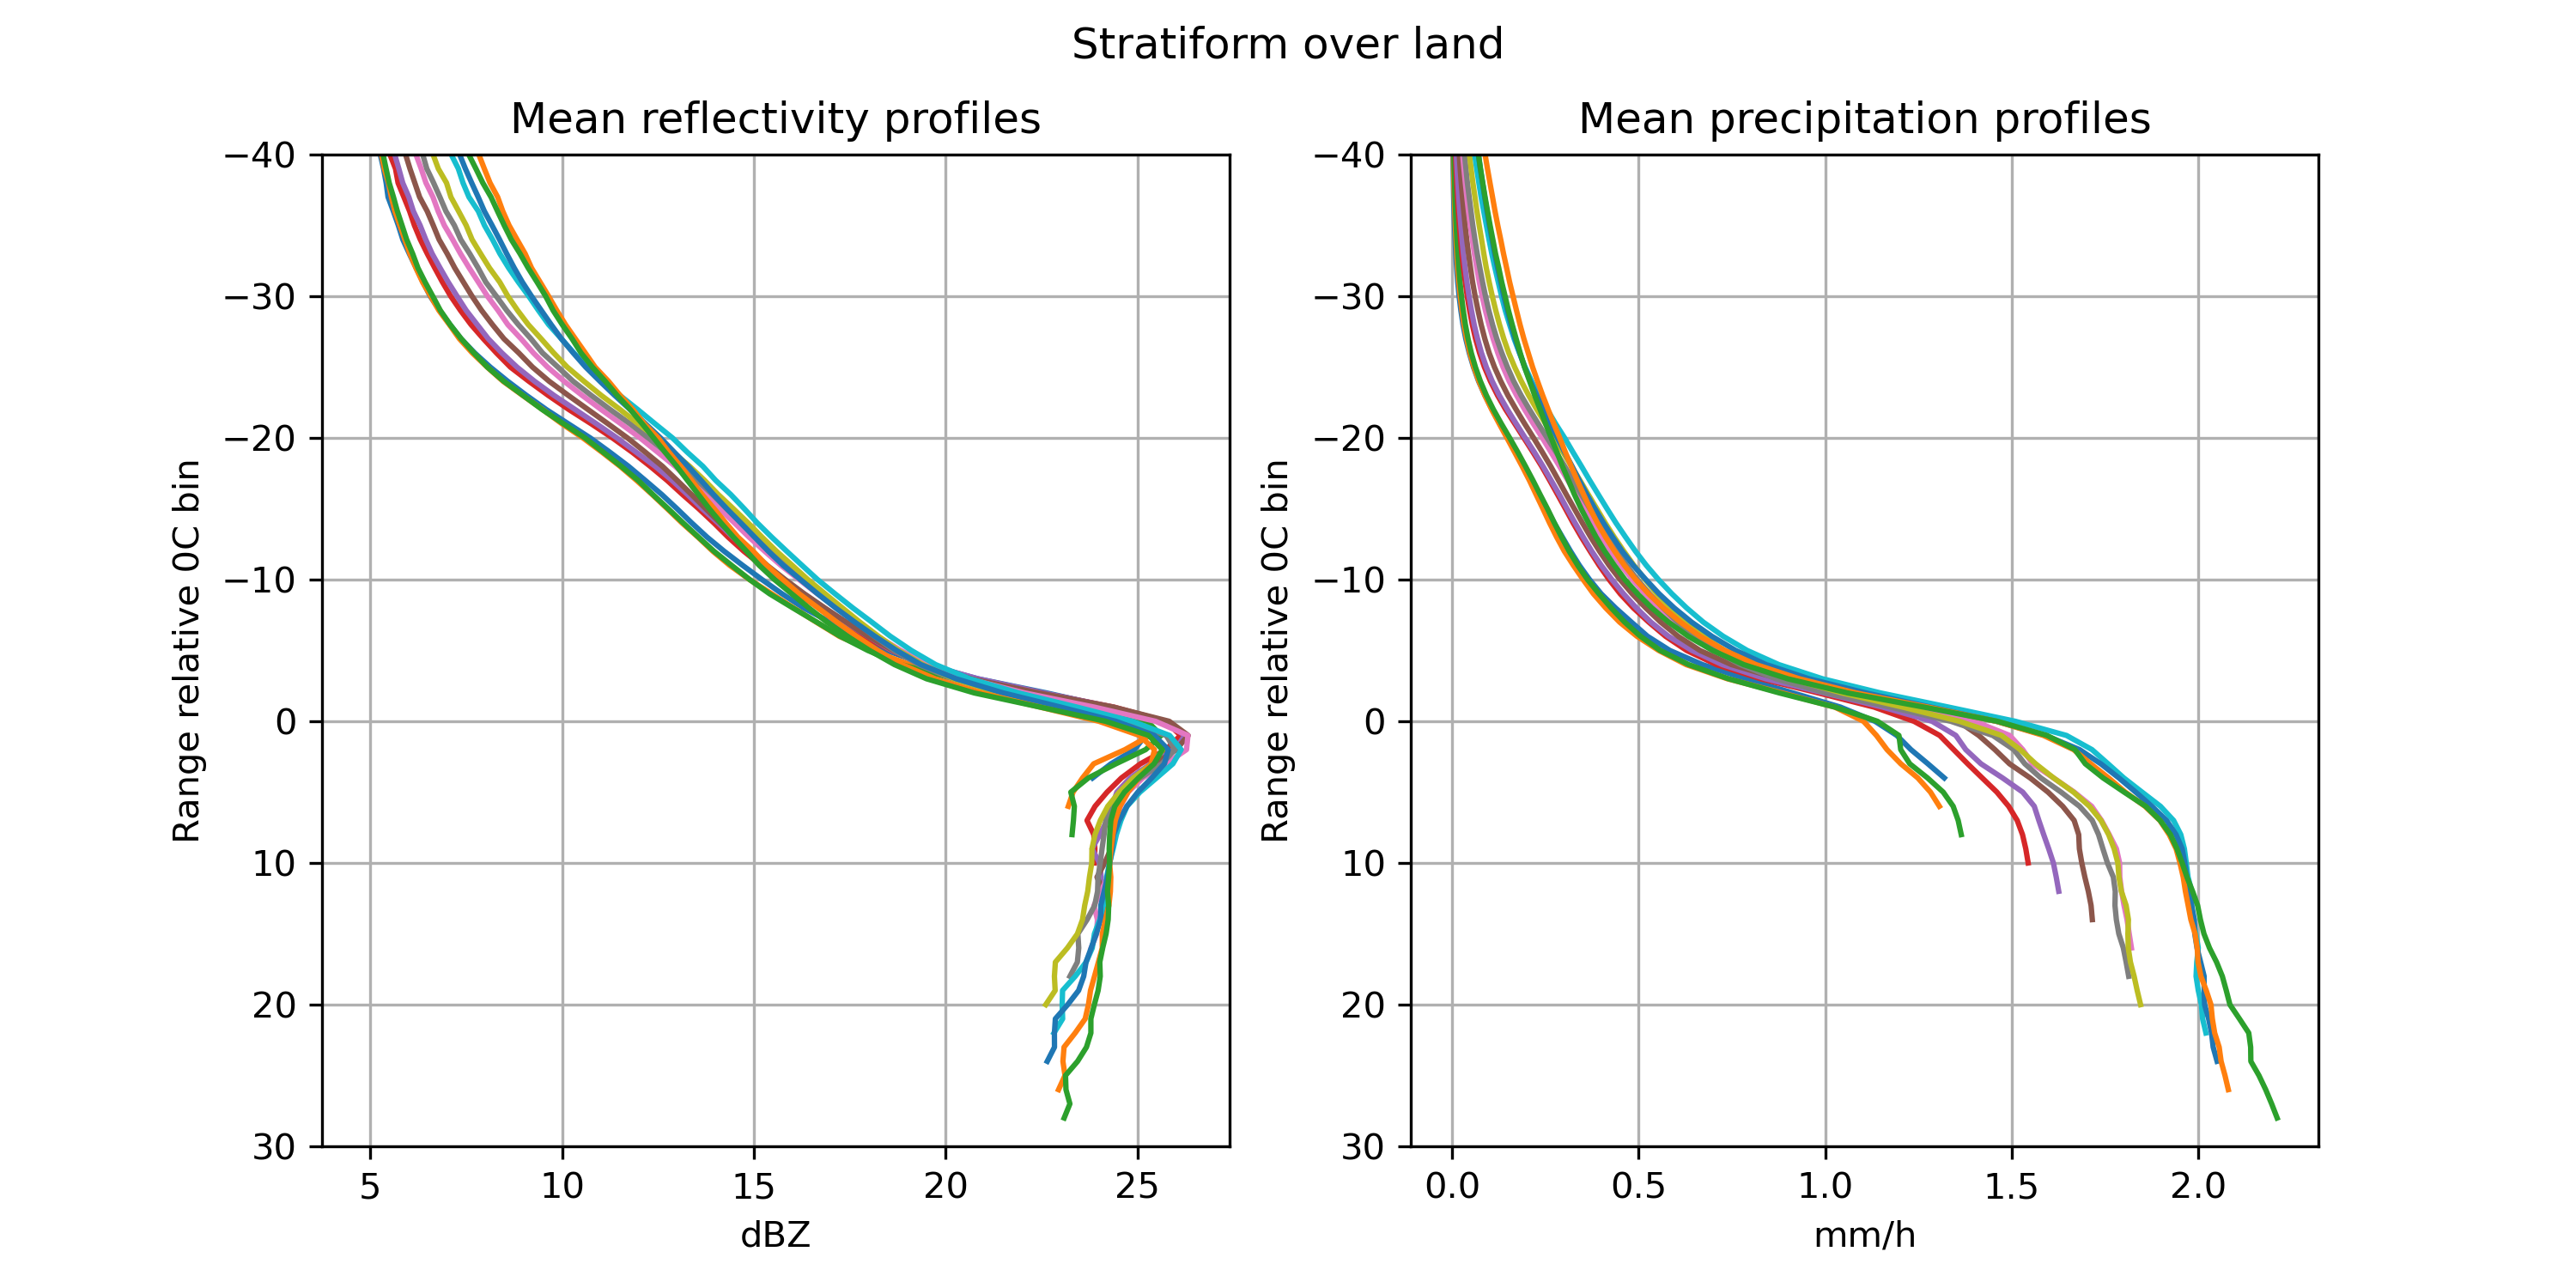
\includegraphics[width=0.85\textwidth]{reflectivityProfiles.png}
        \caption{Mean reflectivity and precipitation rate profiles}
        \label{fig:fig1}
    \end{figure}
\subsection*{Science Questions}   
    \begin{itemize}
    \item
      Can we derive DPR surface precipitation estimates more accurate than
      those based on climatologic extrapolations?
    \item
      Are the precipitation rate distributions below the freezing level
      unbiased? Given their impact on estimating the surface precipitation,
      this is an import question to address.
    \end{itemize}
    
    
\section*{Methodology}
\subsection*{Surface precipitation estimation}
    
The simplest method to estimate the precipitation rate at a given height
above the sea level from a precipitation rate at a higher level is to
rescale the higher level value by the ratio of the climatologic mean
precipitation rates at the two levels. Mathematically, this may be
written as
    
    \begin{equation}
    P_{rate}(H_1)=P_{rate}(H_2) \frac {<P_{rate}(H_1)>} {<P_{rate}(H_2)>} 
    \end{equation}

where $P_{rate}$ is the precipitation rate, $H_1$ is the height where the
estimate is needed, but for which no direct measurement is available,
$H_2$ is a height ($H_2>H_1$) where a radar
measurement is available, and operator $<\square>$ denotes the
climatologic mean over a large dataset characterized by the same
freezing level, surface and precipitation type.
    
While simple, the challenge in applying a clutter based correction
methodology based on Eq. (1) is the derivation of the correction factors
$\frac {<P_{rate}(H_1)>} {<P_{rate}(H_2)>}$ for all possible ($H_1$,$H_2$)
pairs. However, because the ground clutter depth is a function of the
scanning incidence angle, estimates of the climatologic correction
factor derived from near-nadir reflectivity observations and
precipitation estimates may be used to mitigate the clutter near the
edges of the swath. Moreover, because the mean reflectivity profiles
appear to be very similar when plotted relative to the 0C isotherm (Fig. 1), it may be postulated that 
$\frac {<P_{rate}(H_{1,0C})>} {<P_{rate}(H_{2,0C})>}$
may be assumed invariant with respect to the freezing level, where
($H_{1,0C},H_{2,0C}$) are heights ($H_1$,$H_2$) expressed
relative to the FL height.
    
The veracity of this hypothesis is tested, at the same time with the
effectiveness of the clutter correction, using near-nadir DPR
precipitation rate products. This is explained in the following
paragraphs.
    
Specifically, one year (i.e. 2018) of DPR observations are processed and
all reflectivity profiles over land characterized by fewer than eight
bins affected by clutter are selected. Additional variables such as the
associated precipitation type, the freezing level height and the
estimated precipitation rates are attached to the selected profiles.
The dataset is partitioned
based on the freezing level height in 12 distinct subsets, with the
freezing level heights of each subset within 125 m of 1.875+$k$*0.25
km with $k$ varying from 0 to 11. This dataset allows for both the
investigation of the postulated
$\frac {<P_{rate}(H_{1,0C})>} {<P_{rate}(H_{2,0C})>}$ invariance and the
effectiveness of various types of clutter mitigation including 
the one based on Eq. (1).
    
As $\frac {P_{rate}(H_1)} {P_{rate}(H_2)}$ may be significantly different from
the ratio of the climatologic rates for individual observations, it is
conceivable that a stratification of $\frac {<P_{rate}(H_1)>} {<P_{rate}(H_2)>}$
based on additional factors such as relative humidity, wind shear, etc.
improve the accuracy of the clutter correction. However, in practice,
these factors may not be estimated reliably either from the DPR
observations or from the NWP products associated with them. It is 
possible though that some of these factors have a distinctive signature
in the distribution of the observed reflectivity above the clutter. It
is therefore possible that a stratification of the observed reflectivity
profiles based on distinctive features such as gradients, magnitude, 
curvature, etc. may result in $\frac {<P_{rate}(H_1)>} {<P_{rate}(H_2)>}$
distributions different from that associated with the entire dataset. 
However, rather than subjectively formulating features and explicitly
stratifying the dataset and analyzing the resulting distributions, we
use a Machine Learning (ML) approach.  The ML approach does not require
the explicit use of Eq. (1) and the stratification of the dataset. Instead,
it requires the organization of the dataset into a design matrix and a
response matrix \cite{bishop2006}. The design matrix is an array of 
reflectivity observations, with each row corresponding to a reflectivity
profile and each column to a reflectivity bin. The response matrix is an
array of precipitation rates, with each row corresponding to the
precipitation rate estimates associated with the reflectivity profiles
in the design matrix. The structured organization of the dataset makes it 
possible to explore multiple ML models with minimum effort and select the
optimal one. While ML models are generally physics-agnostic, in the sense
that they do not explicitly make use of physical laws, they can exploit
physical causality embedded in the dataset. For example, if gradients in
the reflectivity profiles above the clutter are reliable
predictors of the precipitation rate at the surface, then an 
ML model based on the k-nearest neighbors (k-NN) algorithm \cite{bishop2006}
will be able to exploit this causality because the nearest neighbors of
a given reflectivity profile are likely to have similar gradients. 
Therefore, there is no need to explicitly incorporate physical intuition
based features in the design matrix, as such features are implicitly
used in the estimation process.  At the same time, physical-based 
features not intuitively obvious may exist. It is therefore beneficial to
consider multiple ML methods and a standardized input and output format 
rather than extending the input with intuition-based features.%%, which but at
%%the same time structurally limiting the estimation process.

In this study we use several ML architectures from the scikit-learn library 
\citep{pedregosa2011}.  These include: the k-NN, the gradient boosting
\citep{friedman2001}, and the random forest \citep{ho1995} architectures.
At the same time, we use the Tensorflow \citep{tensorflow2016}, which is a deep learning
\citep{deepL2016} ML open-source library.

As previously described, the DPR dataset is sorted by the FL height and
characterized by fewer than eight bins affected by ground clutter. As such,
bin 168 in the selected profiles is always clutter-free. For a given 
freezing level and assumed number of bins affected by clutter, i.e. $N_c$,
we set the ML models to predict the precipitation rate associate with 
bin 168 based on the reflectivity observations 
and associated precipitation rates in bins 168-$N_c$ and above.  
Mathematically, this may be expressed as:
\begin{equation}
    P_{rate}(168) = f_{i_{FL},N_c}(\mathbf{P_{rate}(k),Z_m(k)}) 
    \label{eq:ml}
\end{equation}
with $k$ varying from 168-$N_c$ to 168-$N_c$-$N_p$, where $N_p$
is the number of clutter-free bins considered in the estimation. 
The subscript $i_{FL}$ is the bin associated with the 0$^\circ$C isotherm.
While an ML model defined by Eq. (\ref{eq:ml}) may seem limited because
it predicts the precipitation rate at a single bin while we are interested
in predicting the precipitation rate at the surface, it can be used
to predict precipitation rates at bins larger than 168 if the assumed
$\frac {<P_{rate}(H_{1,0C})>} {<P_{rate}(H_{2,0C})>}$ invariance holds. 
In such a case, 
\begin{equation}
    P_{rate}(168+dn) = f_{i_{FL}-dn,N_c}(\mathbf{P_{rate}(k),Z_m(k)}) 
    \label{eq:ml2}
\end{equation}
with $k$ varying from 168-$N_c$ to 168-$N_c$-$N_p$ may be used to predict
the precipitation rate at bin 168+$dn$ where $dn$ is the difference between
the surface bin and 168. The interpretation of Eq. (\ref{eq:ml2}) is that,
under the assumed invariance, precipitation profiles with higher freezing
levels (and implicitly lower 0$^\circ$C isotherm bins) may be used
to predict precipitation rates at bins larger than 168.  The assumed 
invariance may be tested by training and comparing the agreement between
models of types $f_{i_{FL},N_c}(\mathbf{P_{rate}(k),Z_m(k)})$ and 
$f_{i_{FL}-dn,N_c}(\mathbf{P_{rate}}(\mathbf{k}-dn),\mathbf{Z_m}(\mathbf{k}-dn))$
for various $dn$ and $N_c$ values.  Agreement between the two models would
be indicative of the invariance holding. In plain English, that would mean
that a model trained using observations profiles with a higher 
freezing level would perform similarly to one trained using observations
with the same freezing level as the real one. The equivalence is
relative to the 0$^\circ$C isotherm bin,  but would enable extrapolation
to bins larger than 168. 

The scikit-learn library provides a convenient interface to train and
test ML models.  As such, the definition of the scikit-learn ML models
require minimal specifications. They include the number of neighbors
for the k-NN model, the number of trees for the random forest model,
and the number of estimators for the gradient boosting model.  We use
the default values for these parameters and tune them using 
trial and error.  The Tensorflow library, on the other hand, requires
more specific definition of the model architecture.  We use a simple 
fully connected feed forward neural network with two hidden layers. 
The number of neurons in is set to 32 in both hidden layers.  The
activation function is the rectified linear unit (ReLU) \citep{relu2010}
and the output layer is a linear layer.  The loss function is the mean
squared error (MSE) and the optimizer is the Adam optimizer 
\citep{adam2014}. The Tensorflow model is included in the study to
provide insight into how the complexity of the ML model affects the
performance.  Specifically, while the scikit-learn models are relatively
simple, the Tensorflow model is more complex \citep{deepL2016} and may 
be able to capture
more complex relationships between the reflectivity above the
clutter and surface precipitation rate.  

To evaluate the performance of the ML models, we use a cross-validation
approach.  Specifically, the DPR dataset is randomly split into a training and 
a testing dataset with 70\% of profiles in the training dataset and the
remaining 30\% in the testing dataset.  The training dataset is used to 
train the ML models, while the testing dataset is used to evaluate them.


\subsection*{Vertical distributions}

\section*{Results}


%% make 2x2 table
\begin{center}
\begin{figure}
\begin{tabular}{cc}
    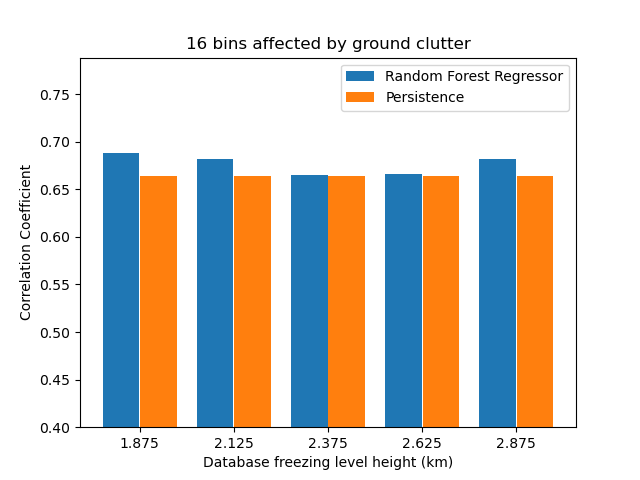
\includegraphics[width=0.495\textwidth]{Figs/corrCoeff_16bins.png}
    &
    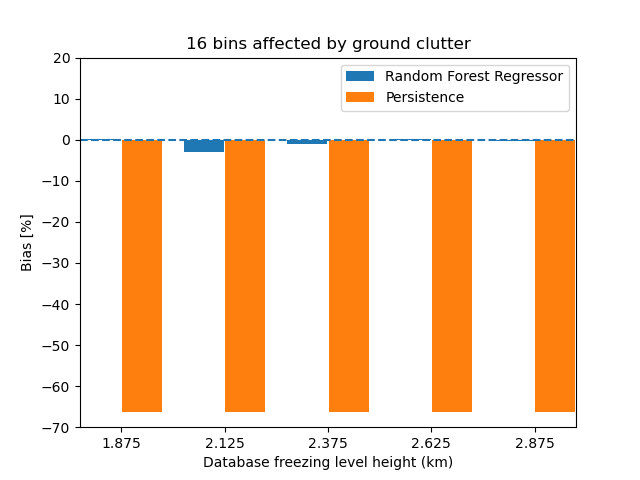
\includegraphics[width=0.495\textwidth]{Figs/bias_16bins.png}\\

    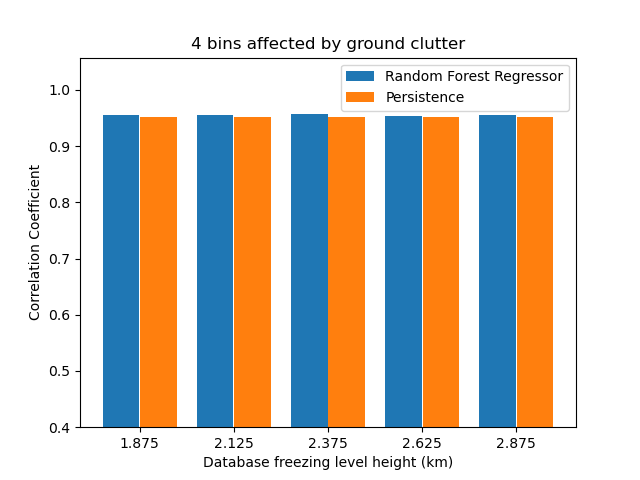
\includegraphics[width=0.495\textwidth]{Figs/corrCoeff_04bins.png}
    &
    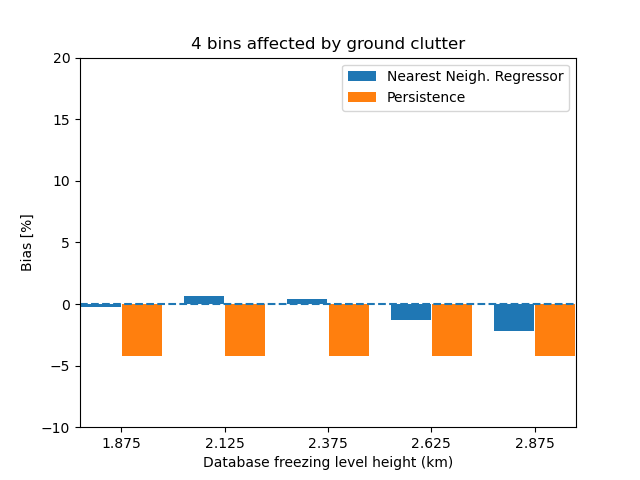
\includegraphics[width=0.495\textwidth]{Figs/bias_04bins.png}\\ 
\end{tabular}
\caption{Performance of a random forest based clutter correction method.}
\end{figure}
\end{center}


\bibliography{references}
\bibliographystyle{plain}
    
\end{document}